% Options for packages loaded elsewhere
\PassOptionsToPackage{unicode}{hyperref}
\PassOptionsToPackage{hyphens}{url}
%
\documentclass[
  ignorenonframetext,
  aspectratio=169]{beamer}
\usepackage{pgfpages}
\setbeamertemplate{caption}[numbered]
\setbeamertemplate{caption label separator}{: }
\setbeamercolor{caption name}{fg=normal text.fg}
\beamertemplatenavigationsymbolsempty
% Prevent slide breaks in the middle of a paragraph
\widowpenalties 1 10000
\raggedbottom
\setbeamertemplate{part page}{
  \centering
  \begin{beamercolorbox}[sep=16pt,center]{part title}
    \usebeamerfont{part title}\insertpart\par
  \end{beamercolorbox}
}
\setbeamertemplate{section page}{
  \centering
  \begin{beamercolorbox}[sep=12pt,center]{part title}
    \usebeamerfont{section title}\insertsection\par
  \end{beamercolorbox}
}
\setbeamertemplate{subsection page}{
  \centering
  \begin{beamercolorbox}[sep=8pt,center]{part title}
    \usebeamerfont{subsection title}\insertsubsection\par
  \end{beamercolorbox}
}
\AtBeginPart{
  \frame{\partpage}
}
\AtBeginSection{
  \ifbibliography
  \else
    \frame{\sectionpage}
  \fi
}
\AtBeginSubsection{
  \frame{\subsectionpage}
}
\usepackage{lmodern}
\usepackage{amssymb,amsmath}
\usepackage{ifxetex,ifluatex}
\ifnum 0\ifxetex 1\fi\ifluatex 1\fi=0 % if pdftex
  \usepackage[T1]{fontenc}
  \usepackage[utf8]{inputenc}
  \usepackage{textcomp} % provide euro and other symbols
\else % if luatex or xetex
  \usepackage{unicode-math}
  \defaultfontfeatures{Scale=MatchLowercase}
  \defaultfontfeatures[\rmfamily]{Ligatures=TeX,Scale=1}
\fi
\usetheme[]{Frankfurt}
\usecolortheme{beaver}
% Use upquote if available, for straight quotes in verbatim environments
\IfFileExists{upquote.sty}{\usepackage{upquote}}{}
\IfFileExists{microtype.sty}{% use microtype if available
  \usepackage[]{microtype}
  \UseMicrotypeSet[protrusion]{basicmath} % disable protrusion for tt fonts
}{}
\makeatletter
\@ifundefined{KOMAClassName}{% if non-KOMA class
  \IfFileExists{parskip.sty}{%
    \usepackage{parskip}
  }{% else
    \setlength{\parindent}{0pt}
    \setlength{\parskip}{6pt plus 2pt minus 1pt}}
}{% if KOMA class
  \KOMAoptions{parskip=half}}
\makeatother
\usepackage{xcolor}
\IfFileExists{xurl.sty}{\usepackage{xurl}}{} % add URL line breaks if available
\IfFileExists{bookmark.sty}{\usepackage{bookmark}}{\usepackage{hyperref}}
\hypersetup{
  pdftitle={Intellectual property rights and International treaties and conventions on use and distribution of genetic resources},
  pdfauthor={Deependra Dhakal},
  hidelinks,
  pdfcreator={LaTeX via pandoc}}
\urlstyle{same} % disable monospaced font for URLs
\newif\ifbibliography
\setlength{\emergencystretch}{3em} % prevent overfull lines
\providecommand{\tightlist}{%
  \setlength{\itemsep}{0pt}\setlength{\parskip}{0pt}}
\setcounter{secnumdepth}{-\maxdimen} % remove section numbering
\usepackage{booktabs}
\usepackage{longtable}
\usepackage{array}
\usepackage{multirow}
\usepackage{wrapfig}
\usepackage{float}
\usepackage{colortbl}
\usepackage{pdflscape}
\usepackage{tabu}
\usepackage{threeparttable}
\usepackage{threeparttablex}
\usepackage[normalem]{ulem}
\usepackage{makecell}
\usepackage{xcolor}
\usepackage{tikz} % required for image opacity change
\usepackage[absolute,overlay]{textpos} % for text formatting

% this font option is amenable for beamer
\setbeamerfont{caption}{size=\tiny}
\newlength{\cslhangindent}
\setlength{\cslhangindent}{1.5em}
\newenvironment{cslreferences}%
  {\setlength{\parindent}{0pt}%
  \everypar{\setlength{\hangindent}{\cslhangindent}}\ignorespaces}%
  {\par}

\title{Intellectual property rights and International treaties and
conventions on use and distribution of genetic resources}
\author{Deependra Dhakal}
\date{}
\institute{Assistant Professor\\
Agriculture and Forestry University\\
\href{mailto:ddhakal.rookie@gmail.com}{\nolinkurl{ddhakal.rookie@gmail.com}}\\
\url{https://rookie.rbind.io/}}

\begin{document}
\frame{\titlepage}

\begin{frame}[allowframebreaks]
  \tableofcontents[hideallsubsections]
\end{frame}
\hypertarget{intellectual-property}{%
\section{Intellectual property}\label{intellectual-property}}

\begin{frame}{Background}
\protect\hypertarget{background}{}
\begin{columns}[T,onlytextwidth]
\column{0.65\textwidth}

\begin{itemize}
\item IP protection consists of principles that a society observes to ensure that an inventor is protected from the unfair use of his/her invention by others.
\item Protection is provisioned in the form of:
  \begin{itemize}
  \footnotesize
  \item Copyright
  \item Patent
  \item Trademark
  \item Trade secret
  \item Breeder's right
  \item Confidential information
  \end{itemize}
\item Innovation has a price tag, hence the investor must be compensated
\item Ensures that invention is not kept secret from betterment of society.
\item Law and science meet here.
\end{itemize}

\column{0.35\textwidth}


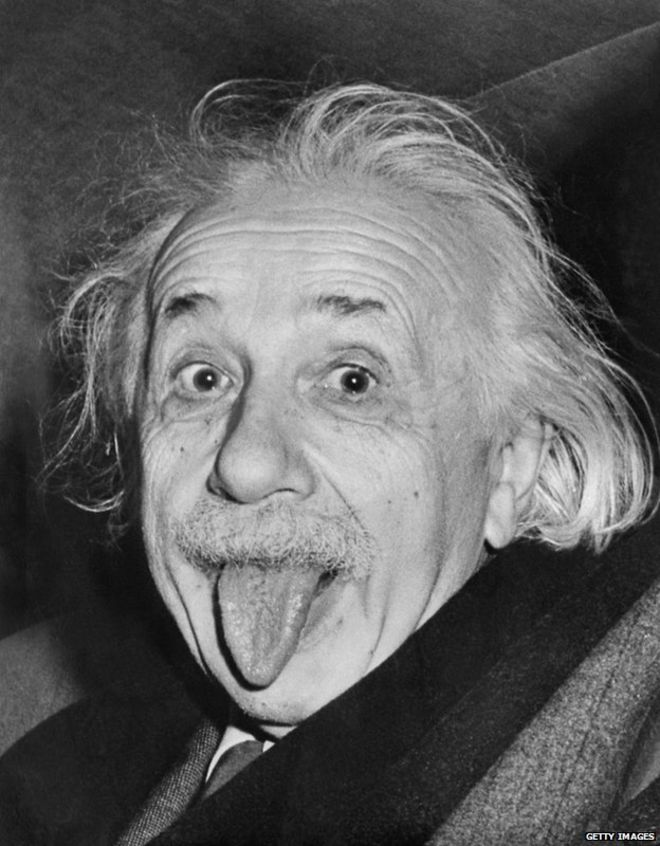
\includegraphics[width=0.9\linewidth]{../images/einstein_ipr} 

\end{columns}
\end{frame}

\begin{frame}{Traditional knowledge}
\protect\hypertarget{traditional-knowledge}{}
\begin{itemize}
\tightlist
\item
  Association between level of biodiversity in a specific region with
  cultural distinctiveness of its inhabitants.
\item
  Specific knowledge of communities living in close relationship to
  their environment: traditional knowledge.
\item
  Integrated into

  \begin{itemize}
  \tightlist
  \item
    Rio Process,
  \item
    International Treaty on PGRFA
  \item
    \href{https://sustainabledevelopment.un.org/milesstones/wssd}{World
    Summit on Sustainable Development}; Johannesburg, South Africa 26
    August - 4 September 2002.
  \end{itemize}
\item
  CBD speaks of `traditional knowledge, innovations and practices of
  indigenous and local communities embodying traditional lifestyles
  relevant for the conservation and sustainable use of biological
  diversity' (Article 8(j)).
\end{itemize}
\end{frame}

\begin{frame}{Traditional knowledge}
\protect\hypertarget{traditional-knowledge-1}{}
\begin{itemize}
\tightlist
\item
  Foster sharing of economic incentives to making available traditional
  knowledge, to conserve it through use, and thereby enhance the
  livelihoods of farming and indigenous communities and reverse the
  decline of biodiversity, upon which, in return, long-term food
  security is based. (Biber-Klemm, Cottier, and others 2006)
\item
  Since the adoption of convention on Biological Diversity (CBD) in
  1992, the law of plant genetic resources (PGR) and the legal status of
  traditional knowledge (TK) has attracted increasing attention.
\item
  2001 Doha Agenda of the WTO explicitly endorsed the issue of
  traditional knowledge as a subject for further work.
\end{itemize}
\end{frame}

\begin{frame}{Traditional knowledge}
\protect\hypertarget{traditional-knowledge-2}{}
\begin{itemize}
\tightlist
\item
  TK has common features for both indigenous as well as farming
  communities:

  \begin{itemize}
  \tightlist
  \item
    Information is not an individual creation, but the achievement of a
    specific community.
  \item
    It cumulates over many generations and evolve accordingly.
  \item
    Managed by and exchanged through customs or customary laws.
  \item
    Close interaction exists between TK and the surrounding ecosystem.
  \end{itemize}
\end{itemize}
\end{frame}

\begin{frame}{Farmer's right}
\protect\hypertarget{farmers-right}{}
\begin{itemize}
\tightlist
\item
  Intellectual contribution of farmers to the diversity of crop
  varieties and animal breeds emphasized in `Farmers' Rights Charter', a
  document drafted by Indian Farmers' Unions.
\item
  Guiding thoughts:

  \begin{itemize}
  \tightlist
  \item
    Farmers ought to have the right to `participate fully in any
    benefits derived from the improved use of these genetic resources'
    and, of course, in the ITPGRFA (Preamble para. 7 and Article 9.1).
  \item
    Farmers' innovations take place collectively and cumulatively, and
    that therefore farmers' rights, arising from their role as
    conservators and breeders, are community rights.
  \end{itemize}
\end{itemize}
\end{frame}

\begin{frame}{PBR and varietal description}
\protect\hypertarget{pbr-and-varietal-description}{}
\begin{itemize}
\tightlist
\item
  Based on the concept that new varieties can be accurately recognized
  and maintained as discrete and unique units.
\item
  Most work of description occured during 1940s and 60s {[}Encyclopedia
  of grain science, page 459{]}.
\item
  During ensuing period, synonyms and homonyms, and varietal piracy we
  belaguering seed and variety use and regulation system.
\item
  Application for PBR necessitates varietal description using plant or
  grain characteristics.
\end{itemize}
\end{frame}

\begin{frame}{}
\protect\hypertarget{section}{}
\begin{itemize}
\tightlist
\item
  Morphological description is important for:

  \begin{itemize}
  \tightlist
  \item
    The award of PBR and tests for distinctness, uniformity and
    stability (DUS);
  \item
    The control of seed production by certification to ensure seed sold
    for agricultural production is true to the variety it is claimed to
    be; and
  \item
    The control of variety purity at the point of final sale, e.g., from
    the farm to the food processor.
  \end{itemize}
\end{itemize}
\end{frame}

\begin{frame}{Tests for DUS}
\protect\hypertarget{tests-for-dus}{}
\begin{itemize}
\tightlist
\item
  Laboratory of field based tests determine whether or not the rights
  are granted.
\item
  To be granted PBR, new variety must be:

  \begin{itemize}
  \tightlist
  \item
    novel -- new to the market, i.e., not available commercially usually
    before the date of application for DUS tests;
  \item
    distinct -- have a unique identity. a consistent difference of at
    least 1 scale point in morphological characters from the most
    similar variety is usually enough to confer distinctness;
  \item
    uniform -- must be sufficiently uniform within the limits achievable
    of the species breeding system, e.g., self-pollinating or partially
    out-pollinating or obligate out-pollinating etc., from which the new
    variety was derived; and
  \item
    stable -- capable of reproducing its uniqueness and uniformity over
    successive generations.
  \end{itemize}
\end{itemize}
\end{frame}

\begin{frame}{Tests for DUS}
\protect\hypertarget{tests-for-dus-1}{}
\begin{itemize}
\tightlist
\item
  Usually for 2 successive growing seasons.
\item
  The UPOV guidelines specify which characters should be recorded, at
  what growth stage records should be taken, the states of expression of
  individual characters, and example varieties that illustrate specific
  states of expression
\item
  For SP cereals, once practical homozygosity is reached, variety enters
  into DUS tests and performance trials.

  \begin{itemize}
  \tightlist
  \item
    What percent of applications should then meet uniformity criteria ?
  \item
    Distinctness is measured by recording morphological characters on
    1-9 scale. One being the weakest state of expression. For example
    anthocyanin color of the leaf margins in corn. Distinctness may show
    discrete expression too. Presence of hairs on rachilla of barley.
  \end{itemize}
\end{itemize}
\end{frame}

\begin{frame}{}
\protect\hypertarget{section-1}{}
\begin{table}

\caption{\label{tab:uk-cereal-breeding}Varietal breeding program in UK}
\centering
\fontsize{6}{8}\selectfont
\begin{tabular}[t]{>{\raggedright\arraybackslash}p{3em}>{\raggedright\arraybackslash}p{5em}>{\raggedright\arraybackslash}p{20em}>{\raggedright\arraybackslash}p{24em}}
\toprule
Year & Generation & Activity & Selection\\
\midrule
\textbf{\cellcolor{gray!6}{1}} & \cellcolor{gray!6}{Initial cross} & \cellcolor{gray!6}{Malting quality x disease resistance} & \cellcolor{gray!6}{Choice of parents often based upon existing varieties that are commercially successful}\\
\textbf{2} & F1 &  & \\
\textbf{\cellcolor{gray!6}{3}} & \cellcolor{gray!6}{F2} & \cellcolor{gray!6}{2000 single plants} & \cellcolor{gray!6}{Selection for disease resistance by deliberate infection}\\
\textbf{4} & F3 and F4 & 100 lines from selected plants & F4 grown in Australia/New Zealand to achieve two generations in one harvest year, micromating selection tests.\\
\textbf{\cellcolor{gray!6}{5}} & \cellcolor{gray!6}{F5} & \cellcolor{gray!6}{8 lines from selected plants} & \cellcolor{gray!6}{Replicated yield trials, malting tests, purification using morphology and protein electrophoresis.}\\
\addlinespace
\textbf{6} & F6 & 4 lines & Further yield trials; Purification using morphology\\
\textbf{\cellcolor{gray!6}{7}} & \cellcolor{gray!6}{F7} & \cellcolor{gray!6}{Plants from lines harvested and grown as plant or ear rows; harvested seed bulked} & \cellcolor{gray!6}{Final breeders performance evaluation trials; purification by morphology/protein electrophoresis; seed bulked for official tests and trials}\\
\textbf{8} & F8 & First year of official tests and trials & Purification based on morphology to prepare seed for commercial seed production\\
\textbf{\cellcolor{gray!6}{9}} & \cellcolor{gray!6}{} & \cellcolor{gray!6}{Second year of official tests and trials} & \cellcolor{gray!6}{Preliminary certification for seed production; purification based on morphology}\\
\textbf{10} &  & Award of PBR; listed for marketing & Enters commercial seed production and official seed certification\\
\addlinespace
\textbf{\cellcolor{gray!6}{11}} & \cellcolor{gray!6}{} & \cellcolor{gray!6}{Further commercial evaluations for marketing} & \cellcolor{gray!6}{Limited seed available to farmers}\\
\textbf{12} &  & Final commercial evaluations for marketing & Seed widely available to meet demand from farmers for new improved variety\\
\bottomrule
\end{tabular}
\end{table}
\end{frame}

\begin{frame}{}
\protect\hypertarget{section-2}{}
\begin{figure}
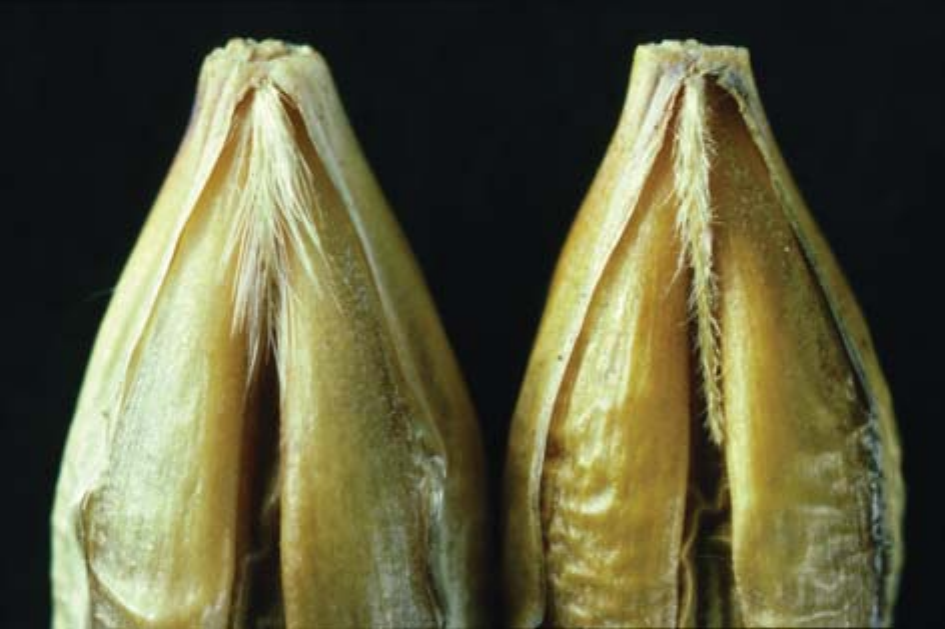
\includegraphics[width=0.45\linewidth]{../images/rachilla_barley} \caption{Differences in barley rachilla hair type: left, long-haired; right, short-haired.}\label{fig:barley-rachilla}
\end{figure}
\end{frame}

\begin{frame}{Varietal descriptors for cereals and grains}
\protect\hypertarget{varietal-descriptors-for-cereals-and-grains}{}
\begin{itemize}
\tightlist
\item
  Seasonal type; Spring, winter, summer
\item
  Early growth characters; Prostrate, erect, hairs on lower leaf sheath,
  coleoptile anthocyanin.
\item
  Leaf characteristics; Color, size, leaf attitude, auricles
\item
  Ear emergence\footnote<.->{See this post:
    \href{https://rookie.rbind.io/post/valentine-wheat/}{Valentine
    Wheat}}
\item
  Plant height
\item
  Glaucosity
\item
  Anthocyanin pigmentation
\item
  Morphology of ear
\item
  Morphology of grain
\item
  Others: shape of the lodicules, color of aleurone layer, color of
  grain, shape of germ area and embryo, physiological reaction to phenol
  immersion, etc.
\end{itemize}
\end{frame}

\begin{frame}{}
\protect\hypertarget{section-3}{}
\begin{figure}
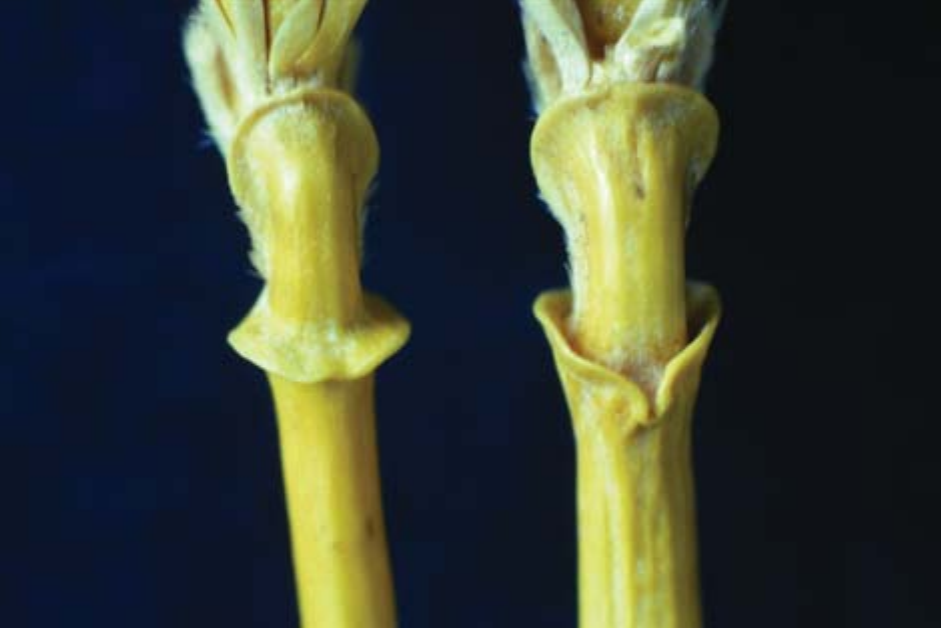
\includegraphics[width=0.45\linewidth]{../images/rachis_barley_collar} \caption{Differences in the 'collar' of the first rachis segment of barley ears: left, 'platform' collar; right, 'cup' collar.}\label{fig:rachis-collar-barley}
\end{figure}
\end{frame}

\begin{frame}{}
\protect\hypertarget{section-4}{}
\begin{columns}[T,onlytextwidth]
  
  \column{0.5\textwidth}

\begin{figure}
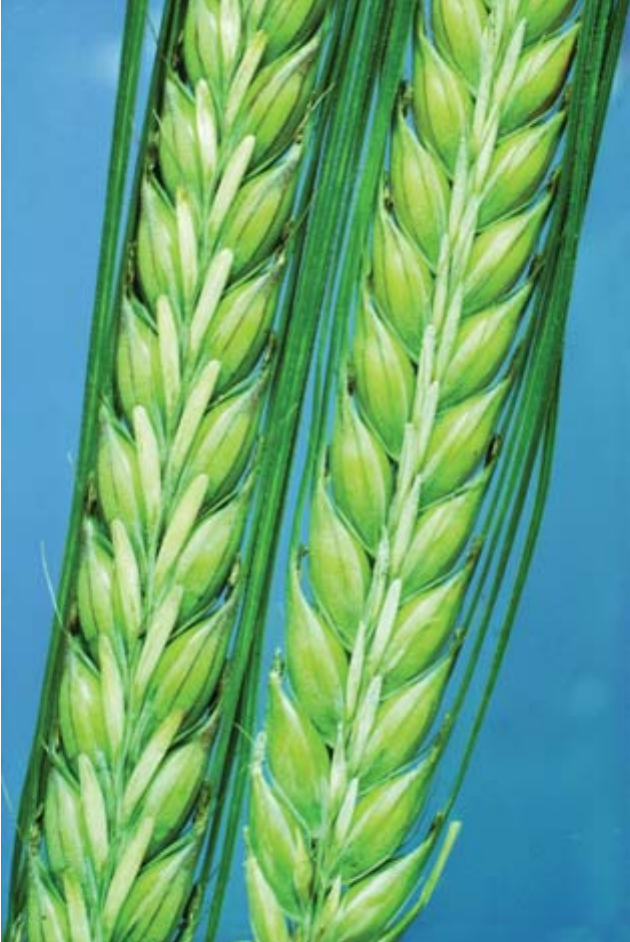
\includegraphics[width=0.55\linewidth]{../images/sterile_spikelets_attitude} \caption{Differences in the attitude of the sterile spikelets of two-row barley: left, sterile spikelets divergent; right, sterile spikelets parallel.}\label{fig:spikelet-attitude}
\end{figure}

  \column{0.5\textwidth}

\begin{figure}
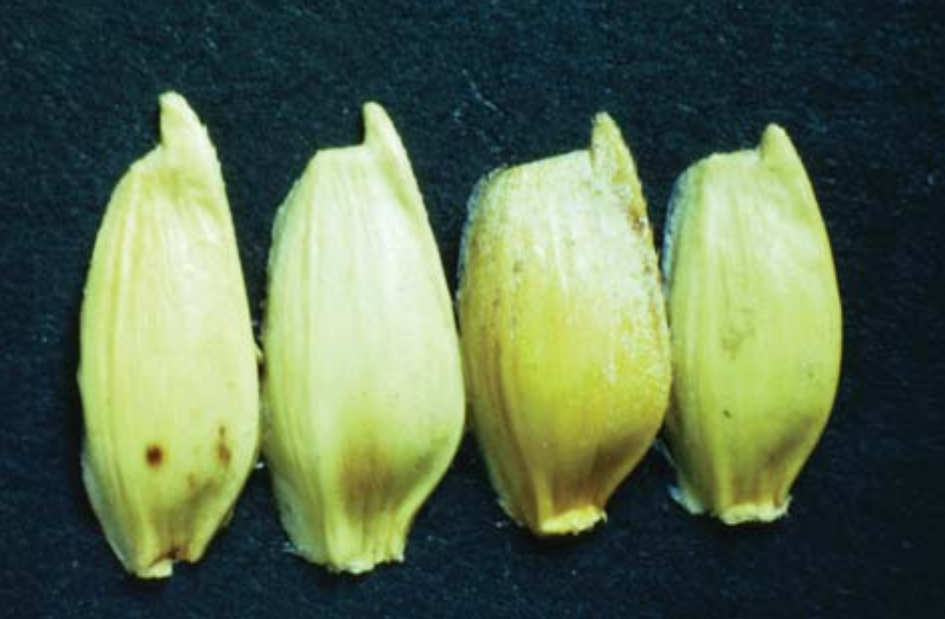
\includegraphics[width=0.75\linewidth]{../images/lower_glumes_wheat} \caption{Contrasting shapes of the lower glume of wheat}\label{fig:shape-lower-glumes}
\end{figure}

\end{columns}
\end{frame}

\hypertarget{international-treaties-conventions-and-organization-on-use-and-distribution-of-genetic-resources}{%
\section{International treaties, conventions and organization on use and
distribution of genetic
resources}\label{international-treaties-conventions-and-organization-on-use-and-distribution-of-genetic-resources}}

\begin{frame}{}
\protect\hypertarget{section-5}{}
\begin{itemize}
\tightlist
\item
  Agreement on Trade related Aspects of Intellectual Property Rights
  (TRIPS Agreement) within the World Trade Organization (WTO) in 1995.
\item
  International Treaty on Plant Genetic Resources for Food and
  Agriculture in (ITPGRFA) 2002.

  \begin{itemize}
  \tightlist
  \item
    Nepal became the party in October 2010.
  \end{itemize}
\item
  World Intellectual Property Organization
  (\href{https://www.wipo.int/portal/en/index.html}{WIPO})
\end{itemize}
\end{frame}

\begin{frame}{UPOV}
\protect\hypertarget{upov}{}
\begin{itemize}
\tightlist
\item
  International Union for the Protection of New Varieties of Plants
  (Union International pour la Protection des Obtentions Vegetales;
  UPOV) was established in 1961.
\item
  It seeks to protect new varieties of plants both in the interest of
  agricultural development and of plant breeders.
\item
  UPOV sought from the outset to provide incentives to the private
  sector to engage in commercial plant breeding, by introducing
  so-called plant breeders' rights, aka. Plant Variety Rights.
\item
  Agreed guidelines for the conduct of tests and standardization of
  variety descriptions based upon the morphology of the grain and plant.
\end{itemize}
\end{frame}

\begin{frame}{}
\protect\hypertarget{section-6}{}
\begin{itemize}
\tightlist
\item
  PBR is an IPR, often described as plant ``patent''
\item
  Breeders can claim royalties on seed sold.
\item
  Once granted, PBR ecognizes the exclusive rights of individual plant
  breeders to produce or reproduce protected varieties, to condition
  them for the purpose of propagation, to offer them for sale, to
  commercialize them, including exporting and importing them, and to
  stock them with a view to production or commercialization (Article
  14.1 UPOV).
\item
  Like any patent right, PBR expires after 20 years.
\end{itemize}
\end{frame}

\begin{frame}{TRIPS}
\protect\hypertarget{trips}{}
\begin{itemize}
\tightlist
\item
  General Agreement on Tariffs and Trade (GATT) contains important
  provisions covering the protection of intellectual property in the
  agreement on Trade Related Aspects of Intellectual Property Rights
  (TRIPS).
\item
  For most member countries ratification of GATT means membership of
  UPOV and a PBR system based upon plant morphology.
\item
  Plant breeders will still use morphological characters to purify
  candidate varieties before submitting them for tests and trials, and
  seed traders will still use morphological characters to verify variety
  at the point of sale.
\item
  However, the science of systematics is being revolutionized by
  molecular technologies.
\item
  Concept of ``Essentially derieved varieties''
\end{itemize}
\end{frame}

\hypertarget{intellectual-property-law}{%
\section{Intellectual property law}\label{intellectual-property-law}}

\begin{frame}{Case study}
\protect\hypertarget{case-study}{}
\begin{itemize}
\tightlist
\item
  Pendragon, a leading mathematician, devised a mathematical formula
  that could be used to draw nonrepeating patterns. Pendragon published
  his formula in mathematics journals, along with several examples of
  patterns drawn using the formula. Pendragon's invention (or perhaps
  discovery) of Pendragon tiling was a significant advance in
  mathematics. Many people took up further study and use of Pendragon's
  ideas. Mathematics departments all over the world began to teach about
  Pendragon patterns, and mathematicians deepened their research in
  advancing the area.
\end{itemize}
\end{frame}

\begin{frame}{}
\protect\hypertarget{section-7}{}
An engineer at Keening Paper read about Pendragon patterns in an article
in Science This Week. The engineer realized that nonrepeating patterns
could have a very useful application in making paper products. When
paper is sold on rolls, one hazard of putting patterns on the paper is
that the paper may stick to the roll if matching patterns are placed one
on top of each other. The use of nonrepeating patterns could reduce this
production flaw. Some nonrepeating patterns would also reduce air
spaces, reducing the size of the paper roll. Shortly thereafter, a
design identical to a design in one of Pendragon's scholarly articles
began to appear on rolls of paper towels made and sold by Keening. That
particular design is just one of millions that could be made by using
Pendragon's formula. Later on, other Keening products appeared with
Pendragon patterns. These designs were not the same as those previously
published by Pendragon. Rather, Keening apparently had used Pendragon's
formula to draw additional designs, rather than simply copying designs
from the work of Pendragon or others.
\end{frame}

\begin{frame}{}
\protect\hypertarget{section-8}{}
Almost two years after Keening started selling such products, Pendragon
learned of this use of his work and consulted his lawyer. He asked her
whether the law prevented the copying of the particular pattern that
Keening had chosen and whether he had the right to prevent Keening from
using his formula to draw other patterns and use them on their products.
\end{frame}

\begin{frame}{Copyright}
\protect\hypertarget{copyright}{}
\small

\begin{itemize}
\tightlist
\item
  Copyright entails the protection of expressions of mental activity not
  only in the arts and sciences, but also in modern technology.
\item
  It does not protect substance, ideas, procedures and methods
  (including mathematical concepts).
\item
  Does not require a high level of originality.
\item
  Copyright and neighbouring rights protection is important for the
  protection of TK to the extent that it is expressed.
\item
  Coverage of copyrights and neighboring rights:

  \begin{itemize}
  \tightlist
  \item
    Traditional music and performances
  \item
    Electronic data collections on PGR
  \item
    Computer programs programming
  \item
    Books and publications
  \item
    Performances and film broadcasts.
  \end{itemize}
\item
  Otherwise, copyright is not suitable for addressing PGR and knowledge
  per se
\item
  Contributes by protecting the cultural background and its diversity.
\end{itemize}
\end{frame}

\begin{frame}{Copyright}
\protect\hypertarget{copyright-1}{}
\begin{itemize}
\tightlist
\item
  Copyright applies to original works of authorship as soon as they are
  fixed in any tangible medium of expression.
\item
  The author of the work initially owns the copyright, although she may
  transfer her rights to others.
\item
  If the work is created by an employee (a work made for hire), the
  author is deemed to be the employer.
\item
  The copyright term lasts for the life of the author plus 70 years (or
  a fixed term of 95 years for works made for hire and some other
  categories of works).
\item
  The copyright owner has the exclusive rights to make copies of the
  work, distribute copies to the public, adapt the work, display the
  work publicly, and perform the work publicly.
\end{itemize}
\end{frame}

\begin{frame}{}
\protect\hypertarget{section-9}{}
Pendragon's scholarly articles and his diagrams of Pendragon tiling
qualify for copyright protection. They qualify as original works of
authorship because they originated with him and easily meet the minimal
standard of creativity required. Pendragon did not register his
copyright. But copyright does not depend on complying with formalities,
such as registering the copyright, depositing copies with the Library of
Congress, or using copyright notices on copies of the work. Such
practices are permitted and offer practical advantages, but they are not
necessary to create the copyright. Rather, an author owns the copyright
in any original work of authorship as soon as she fixes it in some
tangible form (writes down a poem, takes a photograph, records a song,
makes a sculpture).
\end{frame}

\begin{frame}{}
\protect\hypertarget{section-10}{}
Keening Paper apparently did infringe the copyright in one of
Pendragon's designs. It copied the design from his article and sold
copies to the public, thereby infringing the rights to make copies and
to distribute those copies to the public. Keening might contend that
there was no proof that it actually copied the design. But there is
sufficient evidence to support an inference of copying, as opposed to
Keening having made the design independently: The design had been
published, an identical design appeared on Keening's paper product after
Keening took an interest in Pendragon patterns, and the odds that the
designs would coincidentally be identical were very low.
\end{frame}

\begin{frame}{}
\protect\hypertarget{section-11}{}
But Pendragon cannot use the copyrights in his articles and designs to
prevent Keening from using Pendragon's mathematical formula to make its
own patterns. Even if Keening admits that it copied Pendragon's formula
from his work and used it to draw the designs, Keening would not be
liable for copyright infringement. Copyright only protects creative
expression. It does not protect ideas, principles, theories, and the
like. One can freely copy from copyrighted works, if one only copies
unprotected material. So it is not copyright infringement to copy the
facts from a history book or to copy the way a computer program works.
\end{frame}

\begin{frame}{Patent}
\protect\hypertarget{patent}{}
\begin{itemize}
\tightlist
\item
  An exclusive right granted for an invention of a product or process
  that provides an novel way of doing something or offers a new
  technical solution to a problem.
\item
  The \textbf{patentee}.
\item
  Also sensible as ``Negative right''
\item
  Without permission, patented should not be made, used, sold, offered
  for sales and imported.
\item
  The patentee must themself oblige to the existing patent laws.
  \textbf{NO} ``Positive right''.
\item
  TRIPs Agreement has following provisions in place:

  \begin{itemize}
  \tightlist
  \item
    To a large extent, the legal conditions applicable to genetic
    resources and TK on patents.
  \item
    Principle of non-discrimination as to the fields of technology, the
    place of invention, and the country of production (Article 27.1)
  \item
    The minimum term of protection is 20 years (Article 33)
  \end{itemize}
\end{itemize}
\end{frame}

\begin{frame}{Patent}
\protect\hypertarget{patent-1}{}
\begin{itemize}
\tightlist
\item
  Advantages of patents:

  \begin{itemize}
  \tightlist
  \item
    Promotes the progress of science and the useful arts
  \item
    Disclosure of information expands the existing technical knowledge
  \item
    Prestigious to the owner
  \item
    Potential financial value
  \item
    Provides incentives for creativity, innovation, recognizing the
    achievement of investor
  \item
    Fosters private sector contribution/investment.
  \end{itemize}
\item
  Disadvantages of patents:

  \begin{itemize}
  \tightlist
  \item
    Companies find much incentive in improving crops with high market
    potential, whereas those crops with high social values are orphaned
  \item
    Reach-through patents, patent stacking, submarine patent
  \end{itemize}
\end{itemize}
\end{frame}

\begin{frame}{Patent: What can/not be patented?}
\protect\hypertarget{patent-what-cannot-be-patented}{}
\footnotesize

\begin{itemize}
\tightlist
\item
  Patenting involves defining the scope of protection
\item
  Types (units): Utility, Design, Plant
\item
  Types (coverage): National, Transnational
\end{itemize}

\begin{columns}[T,onlytextwidth]
  \footnotesize
  \column{0.5\textwidth}
  Can be patented:
  \begin{enumerate}
  \item Composition of matter
  \item Processes or procedures
  \item Articles of manufacture
  \item Machines
  \item Improvements
  \end{enumerate}
  
  \column{0.5\textwidth}
  Cannot be patented:
  \begin{enumerate}
  \item Ideas and suggestions
  \item Mixtures of ingredients, unless they produce synergistic, unique or unexpected advantage cannot be patented.
  \end{enumerate}
\end{columns}

\begin{columns}[T,onlytextwidth]
  \footnotesize
  \column{0.5\textwidth}
  \vspace{0.8cm}
  Patentability criteria
  \begin{itemize}
  \item Conception
  \item Reduction to practice
  \item Utility
  \end{itemize}
  
  \column{0.5\textwidth}
  \vspace{0.8cm}
  \begin{itemize}
  \item Novelty
  \item Non obviousness
  \end{itemize}
\end{columns}
\end{frame}

\begin{frame}{}
\protect\hypertarget{section-12}{}
Pendragon did not apply for a patent on his formula, so he cannot
exclude others from using it. Even if Pendragon had applied for a
patent, his formula would probably fall outside the scope of patentable
subject matter. The scope of patentable products and processes is very
broad. But certainthings are not patentable, such as the laws of nature,
physical phenomena, and abstract ideas. Pendragon's formula likely would
fall into the category of nonpatentable abstract ideas. Pure mathematics
and other abstractions are not patentable. Rather, to be patentable, an
invention must produce a useful, concrete, and tangible result.
Pendragon might argue that his formula does produce such a result
because it can be used to draw interesting-looking patterns. But when
the formula is not tied to any particular application but instead can be
used to draw millions of patterns that could be used for any number of
purposes, the formula would be deemed too abstract to be patentable.
\end{frame}

\begin{frame}{}
\protect\hypertarget{section-13}{}
Keening, however, did apply the formula to a useful, concrete, and
tangible result. Although Keening did not invent the formula, an
invention may consist of the application or improvement of someone
else's work. Keening used the formula to make paper products that were
less likely to stick to the roll. This invention might have qualified
for a patent. Keening would have been subject to substantive standards
for patentability. These require that the invention be new, useful, and
nonobvious. Keening might well have met the requirement of
nonobviousness, if paper engineers would not have been likely to make
the leap that Keening's engineer did. Likewise, the invention was
sufficiently useful, if it indeed would reduce the problem of paper
sticking to the role. But Keening would not now meet the requirement
that the invention be new. This requirement has two aspects. The
invention was new when Keening first created it, in the sense that it
was unprecedented. But it is no longer new in the other legal sense,
which requires that Keening apply for a patent no later than one year
after the invention is published or in public use. Because Keening has
been selling the product for almost two years, the company has lost its
right (if any) to patent it.
\end{frame}

\begin{frame}{Trademark}
\protect\hypertarget{trademark}{}
\begin{itemize}
\tightlist
\item
  Protection of goods and services in trade
\item
  Trademark protection is of key importance in identifying and
  individualizing products originating from PGR and/or based on TK.
\item
  Seeds and varieties can be sold under trademarks, and TK can be
  protected indirectly by linking it to trade names and supplementary
  qualifications, using terms not in the public domain.
\item
  Functions

  \begin{itemize}
  \tightlist
  \item
    identification of the origin of the product
  \item
    facilitation of consumer to distinguish different products.
  \end{itemize}
\item
  Trademarks cannot be used to bar parallel imports unless there is a
  risk of confusion for the consumer (TRIPS, Article 16.1).
\item
  The term of protection is no less than 7 years, with indefinite
  possibility of renewal (Article 18).
\item
  A possibility of cancellation of trademarks exists only after a
  minimal time period of non-use of 3 years (Article 19).
\end{itemize}
\end{frame}

\begin{frame}{Trademark}
\protect\hypertarget{trademark-1}{}
\begin{itemize}
\tightlist
\item
  A trademark is a symbol used by a person in commerce to indicate the
  source of her goods or services and to distinguish them from those
  sold or made by others.
\item
  The trademark owner acquires trademark rights by making bona fide use
  of the mark in commerce.
\item
  The owner retains ownership of the mark until she abandons use of it.
\item
  Trademark registration offers advantages but is not necessary to
  create a trademark right.
\item
  Unauthorized use of a trademark in a manner that is likely to confuse
  consumers about the source of goods or services infringes the
  trademark.
\item
  Trademark law also provides causes of action beyond trademark
  infringement:

  \begin{itemize}
  \tightlist
  \item
    false designation of origin;
  \item
    false advertising;
  \item
    dilution of famous trademarks; and
  \item
    impermissible registration, use, or trafficking in internet domain
    names that are similar to the trademarks of others.
  \end{itemize}
\end{itemize}
\end{frame}

\begin{frame}{}
\protect\hypertarget{section-14}{}
In the case we considered, Keening did not use Pendragon's name or any
other symbol that falsely indicated an affiliation with Pendragon.
Keening did use one of Pendragon's designs and also used his formula.
But neither were so closely associated with Pendragon as to confuse
consumers about the source of the paper products or to imply Pendragon's
endorsement. With respect to the formula, it is not protectable as a
trademark in any event. Trademarks do not protect functional matter, and
the formula plays a functional role in creating nonrepeating patterns.
\end{frame}

\begin{frame}{Trade secret}
\protect\hypertarget{trade-secret}{}
\begin{itemize}
\tightlist
\item
  Introduced by the TRIPS Agreement and recognized as an IPR (Article
  2).
\item
  The notion of undisclosed information is defined. A secret is
  protected if it is not generally known or readily accessible to
  persons within circles that normally deal with the information.
\item
  Of significance to herbal practitioners and healers in context of TK
\item
  It must have commercial value and is subject to reasonable measures of
  precaution in order to keep the secret (Article 39).
\item
  The TRIPS Agreement establishes the right to take action against
  infringement of trade secrets, including damages to be paid by
  enterprises which knew, or should have known, that the information
  given included trade secrets (Article 39.2, note 10; Article 45).
\item
  It entails an obligation to protect test data concerning
  pharmaceuticals or agricultural chemical products that utilize new
  chemical entities in the course of an approval procedure against
  unfair commercial use (Article 39.3)
\end{itemize}
\end{frame}

\begin{frame}{Trade secret}
\protect\hypertarget{trade-secret-1}{}
A trade secret is information that has economic value from not being
known to or readily ascertainable by those who could gain value from its
use or disclosure and is the subject of reasonable security measures.
Typical trade secrets are customer lists, manufacturing processes,
computer programs, and blueprints for machines, where such information
is kept secret using reasonable security measures. Pendragon's formula
is not a trade secret. Rather than being kept from others through the
use of security measures, the information was freely published.
\end{frame}

\begin{frame}{}
\protect\hypertarget{section-15}{}
\footnotesize

Like Pendragon, Keening did not take any security measures and therefore
cannot have trade secret rights in its application of Pendragon's
formula to paper products. Keening could have tried to exploit the
information as a trade secret. It could have used the formula to produce
the nonrepeating patterns without disclosing that it was using the
formula. For the information to qualify as a trade secret, it would have
to be valuable because it was unknown to Keening's competitors and also
not readily ascertainable. The information was valuable because it made
the paper less likely to stick to the roll and reduced the roll size. So
the question is whether Keening's competitors could have readily figured
out that Keening was using Pendragon's formula. They may well have been
able to do so. If the competitors could discern that Keening had
nonrepeating patterns on its products, a little research might have led
them to the widespread knowledge among mathematicians that Pendragon
patterns would produce such nonrepeating patterns.
\end{frame}

\hypertarget{bibliography}{%
\section{Bibliography}\label{bibliography}}

\begin{frame}{References}
\protect\hypertarget{references}{}
\hypertarget{refs}{}
\begin{cslreferences}
\leavevmode\hypertarget{ref-biber2006rights}{}%
Biber-Klemm, Susette, Thomas Cottier, and others. 2006. \emph{Rights to
Plant Genetic Resources and Traditional Knowledge: Basic Issues and
Perspectives}. CABI.
\end{cslreferences}
\end{frame}

\end{document}
